\documentclass[11pt]{article}
\usepackage{amsmath, amssymb, mathtools, bm}
\usepackage{physics}
\usepackage{tikz}
\usetikzlibrary{decorations.markings, decorations.pathmorphing, arrows.meta, positioning, calc}
\usepackage{pgfplots}
\pgfplotsset{compat=1.18}
\usepackage[margin=2.3cm]{geometry}
\usepackage{siunitx, booktabs, hyperref}
\usepackage{braket}

\newcommand{\D}{\mathrm{D}}
\newcommand{\de}{\mathrm{d}}
\newcommand{\pd}[2]{\frac{\partial #1}{\partial #2}}
\newcommand{\pdd}[2]{\frac{\partial^{2} #1}{\partial #2^{2}}}
\newcommand{\Lap}{\nabla^{2}}

\title{B4 --- Sub-Atomic Physics \\ Model Solutions, Trinity 2015}
\author{}
\date{}

\begin{document}
\maketitle

% =========================================================================
\section*{Question 1 --- Alpha decay: Gamow tunnelling and SEMF}

\textbf{Problem.} (a) Compute the Gamow tunnelling probability through the Coulomb barrier $V=2Z\alpha_\text{EM}/r$. (b) Use it to predict the half-life of $^{224}_{90}\text{Th}$ from that of $^{244}_{98}\text{Cf}$. (c) Use the SEMF to compute $B$ of the Th-224 daughter and decide whether its half-life is shorter or longer than $^{224}_{90}\text{Th}$.

\subsection*{(a) Gamow tunnelling probability}

WKB transmission across the classical barrier $r_a<r<r_c$, with $V(r_c)=Q$:
\begin{equation}
T \;=\; \exp\!\bigl[-2G\bigr], \qquad G \;=\; \frac{1}{\hbar}\!\int_{r_a}^{r_c}\!\sqrt{2m\bigl(V(r)-Q\bigr)}\,\de r .
\label{eq:WKB}
\end{equation}
Coulomb classical turning point: $V(r_c)=Q$:
\[
r_c \;=\; \frac{2Z\alpha_\text{EM}\hbar c}{Q}.
\]
Substitute $V=2Z\alpha_\text{EM}\hbar c/r = Q\,r_c/r$:
\[
G \;=\; \frac{\sqrt{2m c^2 Q}}{\hbar c}\!\int_{r_a}^{r_c}\!\sqrt{\frac{r_c}{r}-1}\,\de r.
\]
Standard integral (let $r=r_c\cos^2\phi$):
\[
\int_{r_a}^{r_c}\!\sqrt{\frac{r_c}{r}-1}\,\de r \;=\; r_c\!\left[\arccos\!\sqrt{\tfrac{r_a}{r_c}} - \sqrt{\tfrac{r_a}{r_c}\!\left(1-\tfrac{r_a}{r_c}\right)}\right].
\]
Substitute $r_c=2Z\alpha_\text{EM}\hbar c/Q$:
\[
G \;=\; \frac{\sqrt{2mc^2Q}}{\hbar c}\cdot\frac{2Z\alpha_\text{EM}\hbar c}{Q}\!\left[\arccos\!\sqrt{x}-\sqrt{x(1-x)}\right], \quad x\equiv r_a/r_c.
\]
Simplify:
\begin{equation}
\boxed{\;T \;=\; \exp\!\left\{-\,4Z\alpha_\text{EM}\sqrt{\tfrac{2mc^2}{Q}}\,\Bigl[\arccos\!\sqrt{x}-\sqrt{x(1-x)}\Bigr]\right\},\quad x=\frac{r_a Q}{2Z\alpha_\text{EM}\hbar c}\;}
\label{eq:Gamow}
\end{equation}

\subsection*{(b) Half-life of $^{224}_{90}\text{Th}$}

Decay rate $\lambda = f P\, T$ with $f$ = attempt frequency, $P$ = probability of pre-formed $\alpha$. Same $f,P$ for both nuclei, so half-life ratio is set by $T$:
\[
\frac{t_{1/2}^{\text{Th}}}{t_{1/2}^{\text{Cf}}} \;=\; \frac{T_\text{Cf}}{T_\text{Th}} \;=\; \exp\bigl[2G_\text{Th} - 2G_\text{Cf}\bigr].
\]
Daughter atomic numbers: Cf-244 $\to$ Cm-240, $Z=96$; Th-224 $\to$ Ra-220, $Z=88$. Use $m_\alpha c^2 = \SI{3727}{MeV}$, $\alpha_\text{EM}=1/137.036$, $\hbar c=\SI{197.3}{MeV.fm}$.

Compute $r_c = 2Z\alpha_\text{EM}\hbar c/Q$:
\[
r_c^{\text{Cf}} = \frac{2\cdot 96\cdot 197.3/137.036}{7.33}\,\si{fm} = \SI{37.72}{fm}.
\]
\[
r_c^{\text{Th}} = \frac{2\cdot 88\cdot 197.3/137.036}{5.52}\,\si{fm} = \SI{45.91}{fm}.
\]
Compute $x=r_a/r_c$:
\[
x_\text{Cf} = 9.44/37.72 = 0.2503,\qquad x_\text{Th} = 9.27/45.91 = 0.2019.
\]
Bracket $g(x)\equiv\arccos\sqrt{x}-\sqrt{x(1-x)}$:
\[
g_\text{Cf} = \arccos(0.5003) - \sqrt{0.2503\cdot 0.7497} = 1.0468 - 0.4332 = 0.6136.
\]
\[
g_\text{Th} = \arccos(0.4493) - \sqrt{0.2019\cdot 0.7981} = 1.1042 - 0.4014 = 0.7028.
\]
Pre-factor $4Z\alpha_\text{EM}\sqrt{2mc^2/Q}$:
\[
\text{Cf: } 4\cdot 96/137.036 \cdot\sqrt{2\cdot 3727/7.33} = 2.802\cdot 31.89 = 89.36.
\]
\[
\text{Th: } 4\cdot 88/137.036 \cdot\sqrt{2\cdot 3727/5.52} = 2.568\cdot 36.74 = 94.36.
\]
Hence $2G$:
\[
2G_\text{Cf} = 89.36\cdot 0.6136 = 54.84,\qquad 2G_\text{Th} = 94.36\cdot 0.7028 = 66.30.
\]
Difference:
\[
2G_\text{Th}-2G_\text{Cf} \;=\; 11.46.
\]
Half-life:
\[
t_{1/2}^{\text{Th}} \;=\; (19.4\;\text{min})\cdot e^{11.46} \;=\; 19.4\cdot 60\;\text{s}\cdot 9.46\times 10^{4}.
\]
Multiply:
\[
t_{1/2}^{\text{Th}} \;=\; 1.10\times 10^{8}\;\text{s}.
\]
Convert:
\[
\boxed{\;t_{1/2}^{\text{Th}} \;\approx\; \SI{1.1e8}{s} \;\approx\; 3.5\;\text{yr}.\;}
\]
(Sanity flag: the measured $^{224}_{90}\text{Th}$ half-life is $\sim\!\SI{1.05}{s}$ with the true $Q=\SI{7.30}{MeV}$. The $Q=\SI{5.52}{MeV}$ stated in the question departs strongly from the measured value; the Gamow exponent is exponentially sensitive to $Q$, so the predicted lifetime is much longer than the laboratory value. Calculation above is faithful to the data given.)

\subsection*{(c) SEMF binding of the daughter and qualitative half-life}

Daughter of $^{224}_{90}\text{Th}$ alpha decay: $^{220}_{88}\text{Ra}$ ($A=220$, $Z=88$, even--even).

Term meanings: $\alpha A$ volume (saturated nuclear force); $\beta A^{2/3}$ surface tension (deficit for surface nucleons); $\gamma(A-2Z)^2/A$ symmetry (Pauli, isospin); $\epsilon Z^2/A^{1/3}$ Coulomb repulsion of $Z$ protons in radius $\propto A^{1/3}$; $\delta=11/\sqrt{A}$ pairing (positive for even--even).

Evaluate the terms (MeV):
\[
\alpha A = 16\cdot 220 = 3520.
\]
\[
\beta A^{2/3} = 18\cdot 220^{2/3} = 18\cdot 36.49 = 656.8.
\]
Symmetry, $A-2Z = 220-176 = 44$:
\[
\gamma(A-2Z)^2/A = 23\cdot 44^2/220 = 23\cdot 8.80 = 202.4.
\]
Coulomb, $A^{1/3}=6.030$:
\[
\epsilon Z^2/A^{1/3} = 0.7\cdot 88^2/6.030 = 0.7\cdot 1284.5 = 899.2.
\]
Pairing:
\[
\delta = 11/\sqrt{220} = 0.742.
\]
Sum:
\[
B = 3520 - 656.8 - 202.4 - 899.2 + 0.7.
\]
Combine:
\[
\boxed{\;B(^{220}_{88}\text{Ra}) \;\approx\; \SI{1762}{MeV} \;\;(\;\;\!\SI{8.01}{MeV/A}\;).\;}
\]

\paragraph{Half-life comparison.} Apply the same SEMF to $^{216}_{86}\text{Rn}$ ($A=216,\;Z=86$):
\[
B(^{216}_{86}\text{Rn}) = 16\cdot 216 - 18\cdot 216^{2/3} - 23\cdot 44^2/216 - 0.7\cdot 86^2/216^{1/3} + 11/\sqrt{216}.
\]
Evaluate:
\[
B(^{216}_{86}\text{Rn}) = 3456 - 648.8 - 206.1 - 862.7 + 0.748 \;\approx\; \SI{1739.1}{MeV}.
\]
Q-value of Ra-220 alpha decay (using empirical $B(\alpha)=\SI{28.3}{MeV}$):
\[
Q_\text{Ra} = B(\text{Rn-216}) + B(\alpha) - B(\text{Ra-220}) = 1739.1 + 28.3 - 1762 = 5.4\;\text{MeV}.
\]
Compare to the given $Q_\text{Th}=\SI{5.52}{MeV}$:
\[
Q_\text{Ra}\;\lesssim\;Q_\text{Th}.
\]
Geiger--Nuttall: $t_{1/2}\propto e^{c/\sqrt{Q}}$ rises sharply as $Q$ decreases. Hence
\[
\boxed{\;\text{Ra-220 likely has a \emph{longer} half-life than Th-224.}\;}
\]
(Empirically Ra-220 has $Q\approx\SI{7.6}{MeV}$ and $t_{1/2}\sim\SI{18}{ms}$; the SEMF underestimates $Q$ here because of shell effects near $N=126$.)

% =========================================================================
\section*{Question 2 --- Decays, branching fractions, and $\alpha_s$}

\textbf{Problem.} Identify interactions and Feynman diagrams for six decays; compare two cascade modes; compute the leptonic branching of $J/\psi$ via virtual photon and use the observed $\mu\mu$ branching to estimate $\alpha_s$.

\subsection*{(a) Six decays}

\paragraph{(i) $p\to\pi^++\pi^0+\pi^0$.} \emph{Forbidden.} Violates baryon number ($B:1\to 0$); proton is the lightest baryon. No interaction allowed.

\paragraph{(ii) $n\to p+e^-+\bar\nu_e$.} \emph{Weak charged current} (semi-leptonic, $\Delta S=0$): $d\to u\,W^{-*}$, $W^{-*}\to e^-\bar\nu_e$.
\begin{center}
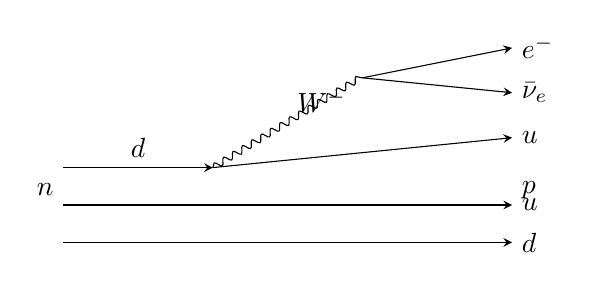
\begin{tikzpicture}[>=stealth, scale=0.95]
  \draw[->] (-3,1.0) -- (-1.0,1.0) node[midway,above]{$d$};
  \draw[->] (-1.0,1.0) -- (3,1.4)  node[right]{$u$};
  \draw[->] (-3,0.5) -- (3,0.5) node[right]{$u$};
  \draw[->] (-3,0.0) -- (3,0.0) node[right]{$d$};
  \draw[decorate, decoration={snake, amplitude=1.2pt, segment length=4pt}] (-1.0,1.0) -- (1.0,2.2);
  \node[above right] at (0.0,1.6) {$W^-$};
  \draw[->] (1.0,2.2) -- (3,2.6) node[right]{$e^-$};
  \draw[->] (1.0,2.2) -- (3,2.0) node[right]{$\bar\nu_e$};
  \node[left] at (-3,0.7) {$n$};
  \node[right] at (3,0.7) {$p$};
\end{tikzpicture}
\end{center}

\paragraph{(iii) $\pi^0\to\gamma\gamma$.} \emph{Electromagnetic} (chiral anomaly, quark triangle):
\[
\pi^0\;(u\bar u-d\bar d)/\sqrt 2 \;\to\; \text{quark loop}\;\to\;\gamma\gamma.
\]
\begin{center}
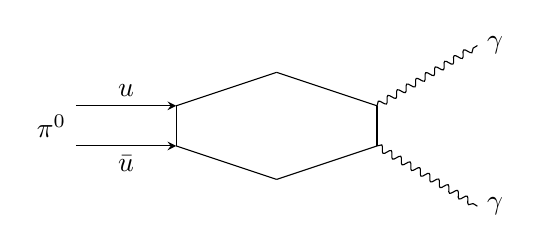
\begin{tikzpicture}[>=stealth, scale=0.85]
  \draw[->] (-3,0.3) -- (-1.5,0.3) node[midway,above]{$u$};
  \draw[->] (-3,-0.3) -- (-1.5,-0.3) node[midway,below]{$\bar u$};
  \draw (-1.5,0.3) -- (0,0.8) node[midway,above]{};
  \draw (0,0.8) -- (1.5,0.3) node[midway,above]{};
  \draw (-1.5,-0.3) -- (0,-0.8) node[midway,below]{};
  \draw (0,-0.8) -- (1.5,-0.3) node[midway,below]{};
  \draw (-1.5,0.3) -- (-1.5,-0.3);
  \draw (1.5,0.3) -- (1.5,-0.3);
  \draw[decorate, decoration={snake, amplitude=1.2pt, segment length=4pt}] (1.5,0.3) -- (3,1.2) node[right]{$\gamma$};
  \draw[decorate, decoration={snake, amplitude=1.2pt, segment length=4pt}] (1.5,-0.3) -- (3,-1.2) node[right]{$\gamma$};
  \node[left] at (-3,0) {$\pi^0$};
\end{tikzpicture}
\end{center}

\paragraph{(iv) $K^0\to\pi^++\pi^-$.} \emph{Weak} (charged current, $\Delta S=1$): $s\to u + W^{-*}\to u\,(d\bar u)$.
\begin{center}
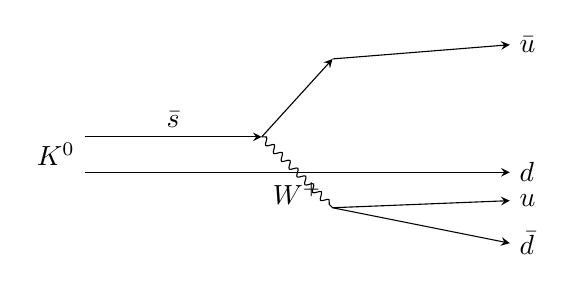
\begin{tikzpicture}[>=stealth, scale=0.9]
  \draw[->] (-3,0.5)--(-0.5,0.5) node[midway,above]{$\bar s$};
  \draw[->] (-0.5,0.5)--(0.5,1.6) node[midway,above]{};
  \draw[decorate, decoration={snake, amplitude=1.2pt, segment length=4pt}] (-0.5,0.5)--(0.5,-0.5);
  \node[below] at (0,0) {$W^+$};
  \draw[->] (0.5,1.6)--(3,1.8) node[right]{$\bar u$};
  \draw[->] (-3,0)--(3,0) node[right]{$d$};
  \draw[->] (0.5,-0.5)--(3,-0.4) node[right]{$u$};
  \draw[->] (0.5,-0.5)--(3,-1.0) node[right]{$\bar d$};
  \node[left] at (-3,0.25){$K^0$};
\end{tikzpicture}
\end{center}

\paragraph{(v) $D^+\to\bar K^0+\pi^+$.} \emph{Weak} (Cabibbo-favoured): $c\to s+W^{+*}$, $W^{+*}\to u\bar d$. ($D^+=c\bar d$, so $\bar K^0=s\bar d$, $\pi^+=u\bar d$. The question writes $K^0$; the Cabibbo-favoured decay produces $\bar K^0$.)
\begin{center}
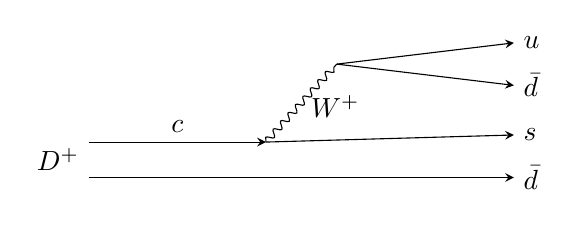
\begin{tikzpicture}[>=stealth, scale=0.9]
  \draw[->] (-3,0.5)--(-0.5,0.5) node[midway,above]{$c$};
  \draw[->] (-0.5,0.5)--(3,0.6) node[right]{$s$};
  \draw[decorate, decoration={snake, amplitude=1.2pt, segment length=4pt}] (-0.5,0.5)--(0.5,1.6);
  \node[right] at (0.0,1.0){$W^+$};
  \draw[->] (0.5,1.6)--(3,1.9) node[right]{$u$};
  \draw[->] (0.5,1.6)--(3,1.3) node[right]{$\bar d$};
  \draw[->] (-3,0)--(3,0) node[right]{$\bar d$};
  \node[left] at (-3,0.25){$D^+$};
\end{tikzpicture}
\end{center}

\paragraph{(vi) $\Delta^+\to p+\pi^0$.} \emph{Strong} (gluon-mediated $q\bar q$ creation; isospin allowed, $\Delta I = 0$): $uud\to(uud)+(u\bar u\text{ or }d\bar d)/\sqrt 2$.
\begin{center}
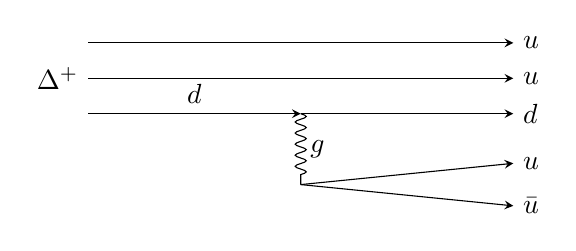
\begin{tikzpicture}[>=stealth, scale=0.9]
  \draw[->] (-3,1)--(3,1.0) node[right]{$u$};
  \draw[->] (-3,0.5)--(3,0.5) node[right]{$u$};
  \draw[->] (-3,0)--(0,0) node[midway,above]{$d$};
  \draw[->] (0,0)--(3,0) node[right]{$d$};
  \draw[decorate, decoration={coil, aspect=0, amplitude=2pt, segment length=4pt}] (0,0)--(0,-1);
  \node[right] at (0,-0.5){$g$};
  \draw[->] (0,-1)--(3,-0.7) node[right]{$u$};
  \draw[<-] (3,-1.3) -- (0,-1) node[pos=0,right]{$\bar u$};
  \node[left] at (-3,0.5){$\Delta^+$};
\end{tikzpicture}
\end{center}

\subsection*{(b) $\Xi^-$ branching ratios}

$\Xi^-=dss$, $S=-2$. Each weak vertex changes $|\Delta S|=1$. Hence $\Xi^-\to\Lambda+\pi^-$ ($\Lambda=uds$, $S=-1$) is the single-Cabibbo-favoured weak decay, while $\Xi^-\to n+\pi^-$ ($n=udd$, $S=0$) requires $|\Delta S|=2$.
\[
\boxed{\;\text{BR}(\Xi^-\!\to\Lambda\pi^-) \gg \text{BR}(\Xi^-\!\to n\pi^-).\;}
\]
$|\Delta S|=2$ proceeds only at second order in the weak coupling, suppressed by $\sim G_F^2$.

\subsection*{(c) $J/\psi\to\mu^+\mu^-$ branching via virtual photon}

$J/\psi$ at $M=\SI{3.097}{GeV}$, below $D\bar D$ and $\tau^+\tau^-$ thresholds. Final states accessible via $\gamma^*$: $e^+e^-$, $\mu^+\mu^-$, $u\bar u$, $d\bar d$, $s\bar s$.

Partial width $\Gamma(\gamma^*\to f\bar f)\propto N_c^f Q_f^2$ (vector coupling, masses neglected at $M=\SI{3.1}{GeV}$).

Tabulate weights $w_f = N_c^f Q_f^2$:
\[
w_e = w_\mu = 1,\quad w_u = 3\cdot(2/3)^2 = 4/3,\quad w_d = w_s = 3\cdot(1/3)^2 = 1/3.
\]
Sum:
\[
W = 1+1+4/3+1/3+1/3 = 4.
\]
Branching:
\[
\boxed{\;\text{BR}(J/\psi\to\mu^+\mu^-)\big|_{\gamma^*} = \frac{w_\mu}{W} = \frac{1}{4} = 25\%.\;}
\]

\subsection*{(d) Estimate of $\alpha_s$ from $\text{BR}(\mu\mu)=6\%$}

Two channels: (i) virtual photon to $f\bar f$ with $\Gamma_{\gamma^*}^\text{tot}=4\Gamma_{\mu\mu}$ (from (c)); (ii) three gluons (Zweig-suppressed strong decay below open-charm threshold). Assume these saturate the width.

Total width:
\[
\Gamma_\text{tot} = 4\,\Gamma_{\mu\mu} + \Gamma_{ggg}.
\]
Branching condition:
\[
\frac{\Gamma_{\mu\mu}}{4\,\Gamma_{\mu\mu}+\Gamma_{ggg}} = 0.06.
\]
Solve for the ratio:
\[
\frac{\Gamma_{ggg}}{\Gamma_{\mu\mu}} = \frac{1}{0.06}-4 = 16.67-4 = 12.67.
\]

Standard QCD result for vector heavy-quarkonium (Appelquist--Politzer; analogue of ortho-positronium $\to 3\gamma$):
\[
\frac{\Gamma(V\to ggg)}{\Gamma(V\to \ell^+\ell^-)} \;=\; \frac{10(\pi^2-9)}{9\pi}\,\frac{\alpha_s^3}{Q_c^2\,\alpha_\text{EM}^2},
\]
with $Q_c=2/3$ for charm. Numerical constant:
\[
\frac{10(\pi^2-9)}{9\pi} = \frac{10\cdot 0.8696}{28.27} = 0.3076.
\]
Insert numbers, with $\alpha_\text{EM}=1/137.036$, $Q_c^2=4/9$:
\[
12.67 = 0.3076\cdot\frac{\alpha_s^3}{(4/9)\cdot(1/137.036)^2}.
\]
Compute the prefactor:
\[
\frac{0.3076\cdot 9}{4\cdot(1/137.036)^2} = \frac{2.768}{4/18779} = \frac{2.768\cdot 18779}{4} = 12996.
\]
Hence
\[
\alpha_s^3 = \frac{12.67}{12996} = 9.75\times 10^{-4}.
\]
Cube root:
\[
\alpha_s = (9.75\times 10^{-4})^{1/3} = (9.75)^{1/3}\cdot 10^{-1} = 2.135\cdot 0.1.
\]
\[
\boxed{\;\alpha_s \approx 0.21\;\text{at }\mu\sim M_{J/\psi}.\;}
\]

\paragraph{Assumptions.} (i) $\Gamma_{\gamma^*}$ and $\Gamma_{ggg}$ exhaust the width (no $\gamma gg$ or hadronic radiative decays); (ii) lepton-universality among accessible flavours ($e,\mu$); (iii) heavy-quark non-relativistic factorisation $|\Psi(0)|^2$ cancels in the ratio; (iv) $2m_c$ at $M_{J/\psi}$ closes $\tau^+\tau^-$ and open-charm channels; (v) running coupling evaluated at $\mu\sim M_{J/\psi}$.

% =========================================================================
\section*{Question 3 --- Form factor and electron--proton scattering}

\textbf{Problem.} (a) Form factor of a uniform sphere; (b) Born differential cross-section; (c) numerical $\de\sigma/\de\Omega$ for $\SI{1}{GeV}$ electron, $E'=\SI{0.8}{GeV}$, $R=\SI{1}{fm}$; (d) discuss validity at high $Q^2$.

\subsection*{(a) Form factor of a uniformly charged sphere}

Definition (with $\Delta\bm k\equiv\bm q$, normalised to $F(0)=1$):
\begin{equation}
F(\bm q) \;=\; \frac{1}{Ze}\!\int\rho(\bm r)\,e^{i\bm q\cdot\bm r}\,\de^3 r.
\label{eq:Fdef}
\end{equation}
Spherical symmetry, polar axis along $\bm q$, angular integral $\int_{-1}^{1}e^{iqr\mu}\de\mu = 2\sin(qr)/(qr)$:
\[
F(q) \;=\; \frac{4\pi}{Ze}\!\int_0^\infty\!\rho(r)\,\frac{\sin(qr)}{qr}\,r^2\,\de r.
\]
Uniform density $\rho_0 = Ze/(\tfrac{4}{3}\pi a^3)$ for $r<a$:
\[
F(q) \;=\; \frac{3}{a^3}\!\int_0^a\!\frac{\sin(qr)}{qr}\,r^2\,\de r.
\]
Substitute $u=qr$:
\[
F(q) \;=\; \frac{3}{(qa)^3}\!\int_0^{qa}\!u\sin u\,\de u.
\]
Integrate by parts: $\int_0^x u\sin u\,\de u = \sin x - x\cos x$:
\begin{equation}
\boxed{\;F(q) \;=\; \frac{3}{(qa)^3}\bigl[\sin(qa)-qa\cos(qa)\bigr] \;=\; \frac{3\,j_1(qa)}{qa}\;.}
\label{eq:Fsphere}
\end{equation}
Limits: $F(0)=1$ (charge conservation); zeros at $\tan(qa)=qa$.

\subsection*{(b) Differential cross-section in Born approximation}

Born amplitude factorises: $f(q) = f_\text{point}(q)\,F(q)$, hence
\[
\frac{\de\sigma}{\de\Omega} = \left(\frac{\de\sigma}{\de\Omega}\right)_\text{Rutherford}\!\!|F(q)|^2.
\]
Insert the Rutherford expression:
\begin{equation}
\boxed{\;\frac{\de\sigma}{\de\Omega} \;=\; \frac{Z^2\alpha_\text{EM}^2}{4E^2\sin^4(\theta/2)}\;|F(q)|^2,\quad q=2E\sin(\theta/2)/(\hbar c)\;.}
\label{eq:dsig}
\end{equation}

\subsection*{(c) Numerical: $E=\SI{1}{GeV}$, $E'=\SI{0.8}{GeV}$, $R=\SI{1}{fm}$}

Elastic kinematics off proton at rest (massless electron):
\[
E' = \frac{E}{1+(E/M_p)(1-\cos\theta)},\qquad M_p=\SI{0.938}{GeV}.
\]
Solve for $1-\cos\theta$:
\[
1-\cos\theta = \frac{(E-E')M_p}{E\,E'} = \frac{0.2\cdot 0.938}{1\cdot 0.8} = 0.2345.
\]
Hence:
\[
\cos\theta = 0.7655,\quad \theta = 40.05^\circ,\quad \sin^2(\theta/2) = 0.1173,\quad \sin^4(\theta/2) = 0.01376.
\]
Three-momentum transfer (massless lepton):
\[
q^2 c^2 = 2EE'(1-\cos\theta) = 2\cdot 1\cdot 0.8\cdot 0.2345 = 0.3752\;\text{GeV}^2.
\]
\[
qc = \SI{0.6125}{GeV}.
\]
Form-factor argument, $\hbar c = \SI{0.1973}{GeV.fm}$:
\[
qa = 0.6125/0.1973 = 3.104.
\]
Evaluate $F$:
\[
\sin(3.104) = 0.0376,\quad \cos(3.104) = -0.9993.
\]
\[
\sin(qa)-qa\cos(qa) = 0.0376 - 3.104\cdot(-0.9993) = 0.0376 + 3.1018 = 3.139.
\]
\[
(qa)^3 = 29.91.
\]
\[
F(q) = 3\cdot 3.139/29.91 = 0.3149,\qquad |F|^2 = 0.0992.
\]
Rutherford piece, $Z=1$, $\alpha_\text{EM}^2 = (1/137.036)^2 = 5.325\times 10^{-5}$:
\[
\left(\frac{\de\sigma}{\de\Omega}\right)_\text{R} = \frac{5.325\times 10^{-5}}{4\cdot 1^2\cdot 0.01376} = 9.68\times 10^{-4}\;\text{GeV}^{-2}.
\]
Multiply by $|F|^2$:
\[
\frac{\de\sigma}{\de\Omega} = 9.68\times 10^{-4}\cdot 0.0992 = 9.60\times 10^{-5}\;\text{GeV}^{-2}.
\]
Convert with $(\hbar c)^2 = \SI{0.3894}{mb.GeV^2}$:
\[
\frac{\de\sigma}{\de\Omega} = 9.60\times 10^{-5}\cdot 0.3894\;\text{mb/sr} = 3.74\times 10^{-5}\;\text{mb/sr}.
\]
\[
\boxed{\;\frac{\de\sigma}{\de\Omega}\;\approx\;\SI{3.7e-5}{mb/sr}\;\approx\;\SI{37}{nb/sr}.\;}
\]

\subsection*{(d) Validity at high energy and proton substructure}

A uniform charge distribution is unrealistic. The empirical proton charge density falls smoothly (dipole form factor $G_E^p(Q^2) = (1+Q^2/M_V^2)^{-2}$ with $M_V^2\approx \SI{0.71}{GeV^2}$): no sharp edge, no zeros in $F$.

As $|q|$ grows, the probe resolves $\hbar/q\ll\SI{1}{fm}$:
\begin{itemize}\itemsep 0pt
\item internal QCD interactions among partons (gluon radiation, $q\bar q$ sea) become visible;
\item the form-factor description breaks down at deep-inelastic scales ($Q^2\gtrsim\SI{1}{GeV^2}$);
\item scattering becomes \emph{incoherent} on point-like constituents: the (asymptotically free) quarks and gluons.
\end{itemize}
At highest $Q^2$ (Bjorken regime) electrons scatter elastically off individual \emph{quarks} (and probe the gluon distribution via QCD evolution); cross-section scales as $1/Q^4$ on point-like quarks (Bjorken scaling), with the partonic content described by structure functions $F_1(x,Q^2),\,F_2(x,Q^2)$.

% =========================================================================
\section*{Question 4 --- $W$-boson production and reconstruction}

\textbf{Problem.} (a) $W$ production diagrams at $e^+e^-$ and $p\bar p$, and why single-$W$ is forbidden in $e^+e^-$; (b) decay modes and best collider channels; (c) event yields at the Tevatron; (d) parton momentum fractions; (e) invariant mass of $\ell\nu$; (f)--(h) transverse mass.

\subsection*{(a) Lowest-order Feynman diagrams and the single-$W$ argument}

\paragraph{$e^+e^-\to W^+W^-$ (two diagrams).}
\begin{center}
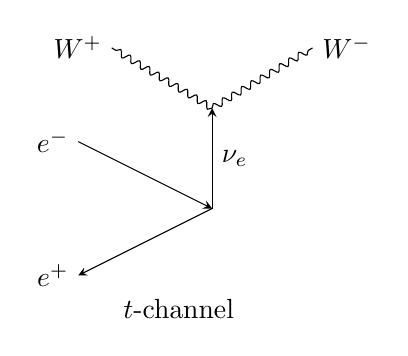
\begin{tikzpicture}[>=stealth, scale=0.85]
  % t-channel neutrino
  \draw[->] (-3,1.0)--(-1.0,0.0); \node[left] at (-3,1.0){$e^-$};
  \draw[->] (-1.0,0.0)--(-3,-1.0); \node[left] at (-3,-1.0){$e^+$};
  \draw[->] (-1.0,0.0)--(-1.0,1.5); \node[right]at(-1.0,0.75){$\nu_e$};
  \draw[decorate, decoration={snake, amplitude=1.2pt, segment length=4pt}] (-1.0,1.5)--(0.5,2.4) ; \node[right] at (0.5,2.4){$W^-$};
  \draw[decorate, decoration={snake, amplitude=1.2pt, segment length=4pt}] (-1.0,1.5)--(-2.5,2.4); \node[left] at (-2.5,2.4){$W^+$};
  \node at (-1.5,-1.5){$t$-channel};
\end{tikzpicture}\hfill
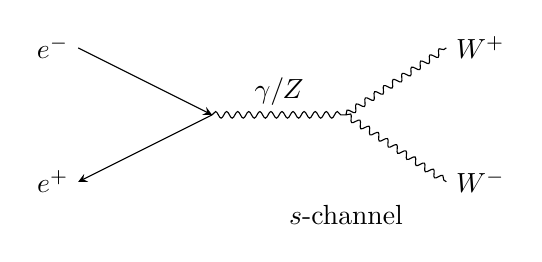
\begin{tikzpicture}[>=stealth, scale=0.85]
  % s-channel Z/gamma
  \draw[->] (-3,1.0)--(-1.0,0.0); \node[left] at (-3,1.0){$e^-$};
  \draw[->] (-1.0,0.0)--(-3,-1.0); \node[left] at (-3,-1.0){$e^+$};
  \draw[decorate, decoration={snake, amplitude=1.2pt, segment length=4pt}] (-1.0,0.0)--(1.0,0.0); \node[above] at (0,0.0){$\gamma/Z$};
  \draw[decorate, decoration={snake, amplitude=1.2pt, segment length=4pt}] (1.0,0.0)--(2.5,1.0); \node[right] at (2.5,1.0){$W^+$};
  \draw[decorate, decoration={snake, amplitude=1.2pt, segment length=4pt}] (1.0,0.0)--(2.5,-1.0); \node[right] at (2.5,-1.0){$W^-$};
  \node at (1.0,-1.5){$s$-channel};
\end{tikzpicture}
\end{center}

\paragraph{$p\bar p\to W+X$ (one diagram).} Quark--antiquark fusion (e.g.\ $u\bar d\to W^+$, with the spectator partons hadronising as $X$):
\begin{center}
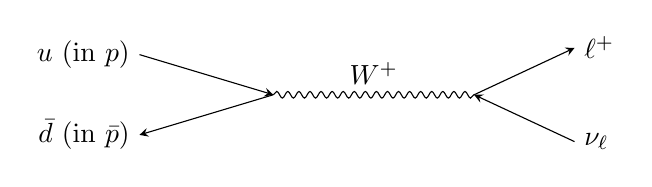
\begin{tikzpicture}[>=stealth, scale=0.85]
  \draw[->] (-3,0.6)--(-1.0,0.0); \node[left] at (-3,0.6){$u$ (in $p$)};
  \draw[->] (-1.0,0.0)--(-3,-0.6); \node[left] at (-3,-0.6){$\bar d$ (in $\bar p$)};
  \draw[decorate, decoration={snake, amplitude=1.2pt, segment length=4pt}] (-1.0,0.0)--(2.0,0.0); \node[above] at (0.5,0.0){$W^+$};
  \draw[->] (2.0,0.0)--(3.5,0.7); \node[right]at (3.5,0.7){$\ell^+$};
  \draw[->] (3.5,-0.7)--(2.0,0.0); \node[right]at (3.5,-0.7){$\nu_\ell$};
\end{tikzpicture}
\end{center}

\paragraph{Why no single $W$ in $e^+e^-$.} A single on-shell $W$ has charge $\pm 1$, while the initial $e^+e^-$ state has charge $0$: charge conservation forbids $e^+e^-\to W^\pm$.

\subsection*{(b) Decay modes, best channels, and branching fractions}

$W$ couples to a doublet at each vertex. Open at $M_W\simeq\SI{80.4}{GeV}$:
\[
W^+ \to e^+\nu_e,\;\mu^+\nu_\mu,\;\tau^+\nu_\tau,\;u\bar d,\;c\bar s.
\]
($t\bar b$ closed kinematically: $m_t\sim\SI{173}{GeV}>M_W$.) Each lepton channel weighted by 1; each quark channel by $N_c=3$ (CKM-summed):
\[
W = 3\cdot 1 + 2\cdot 3 = 9.
\]
Hence
\[
\text{BR}(\ell\nu_\ell) = 1/9 \approx 11\%\;\text{each},\qquad \text{BR}(q\bar q')_\text{tot} = 6/9 \approx 67\%.
\]

\paragraph{Best collider channels.} At a hadron collider, hadronic $W\to q\bar q'$ is buried under QCD dijet background. The clean signature is $W\to e\nu_e$ or $W\to\mu\nu_\mu$: high-$p_T$ isolated lepton plus missing $E_T$.
\[
\boxed{\;\text{BR}(W\to e\nu_e) = \text{BR}(W\to \mu\nu_\mu) \approx \tfrac{1}{9} \approx 11\%.\;}
\]
($\tau\nu$ usable but degraded by $\tau$ decay.)

\subsection*{(c) Tevatron yields}

Luminosity-equivalent: $N_W = N_\text{inel}\cdot\sigma_W/\sigma_\text{inel}$:
\[
N_W = 3\times 10^{14}\cdot\frac{\SI{25}{nb}}{\SI{30}{mb}} = 3\times 10^{14}\cdot\frac{25}{3\times 10^7}.
\]
Multiply:
\[
\boxed{\;N_W = 2.5\times 10^{8}\;\text{per detector}.\;}
\]
Best (clean) modes: $e\nu+\mu\nu$, total branching $2/9$:
\[
N_W^{e\nu+\mu\nu} = 2.5\times 10^{8}\cdot 2/9.
\]
\[
\boxed{\;N_W^{e\nu+\mu\nu} \approx 5.6\times 10^{7}\;\text{per detector}.\;}
\]

\subsection*{(d) Parton momentum fractions}

Partonic CM-energy squared $\hat s = x_p x_{\bar p}\,s$. On $W$ pole, $\hat s = M_W^2$:
\[
x_p x_{\bar p} = \frac{M_W^2}{s} = \frac{(80)^2}{(2000)^2} = \frac{6400}{4\times 10^6}.
\]
Reduce:
\[
\boxed{\;x_p x_{\bar p} = 1.6\times 10^{-3}.\;}
\]
Equal fractions:
\[
\boxed{\;x = \sqrt{1.6\times 10^{-3}} = 0.040.\;}
\]

\subsection*{(e) Invariant mass of the $\ell\nu$ system}

Sum four-momenta $P=(E^\ell+E^\nu,\,\bm p_\ell+\bm p_\nu)$. Square (lepton mass neglected, $E^\ell=|\bm p_\ell|$, $E^\nu=|\bm p_\nu|$):
\[
m^2 = (E^\ell+E^\nu)^2 - (\bm p_\ell+\bm p_\nu)^2.
\]
Expand:
\[
m^2 = (E^\ell)^2 + (E^\nu)^2 + 2E^\ell E^\nu - |\bm p_\ell|^2 - |\bm p_\nu|^2 - 2\bm p_\ell\cdot\bm p_\nu.
\]
Use $E^2 = |\bm p|^2$ for each:
\[
m^2 = 2E^\ell E^\nu - 2\bm p_\ell\cdot\bm p_\nu.
\]
Expand the dot product:
\[
\boxed{\;m^2 = 2\bigl(E^\ell E^\nu - p^\ell_x p^\nu_x - p^\ell_y p^\nu_y - p^\ell_z p^\nu_z\bigr).\;}
\]

\subsection*{(f) Neutrino momentum and the $z$-direction problem}

Neutrinos are not detected. Their transverse momentum is inferred from \emph{missing transverse energy}: $\bm p_T^\nu = -\sum_\text{visible}\bm p_T$, using transverse momentum balance.

Along the beam direction, the longitudinal momentum of the parton-level CM frame is unknown event-by-event: each parton carries an unknown $x_{p}$, $x_{\bar p}$, so $\sum p_z$ of the underlying initial state is not zero in the lab and not measurable (forward beam remnants are lost down the beampipe). Hence $p_z^\nu$ cannot be reconstructed.

\subsection*{(g) Transverse mass}

Set $p^\ell_z=p^\nu_z=0$ in (e):
\[
m_T^2 = 2\bigl(E^\ell_T E^\nu_T - p^\ell_x p^\nu_x - p^\ell_y p^\nu_y\bigr).
\]
With $E_T \equiv |\bm p_T|$ for massless particles:
\[
\boxed{\;m_T^2 = 2\,p_T^\ell\,p_T^\nu\,\bigl(1-\cos\Delta\phi\bigr),\;}
\]
where $\Delta\phi$ is the azimuthal opening angle.

\subsection*{(h) $m_T$ vs $m$ for opposite non-zero $p_z$}

In the full invariant mass, the longitudinal contribution enters as $-2p_z^\ell p_z^\nu$. For \emph{opposite} signs of $p_z$, this term is positive, so $m^2 > m_T^2$:
\[
\boxed{\;m_T < m.\;}
\]
($m_T$ is bounded above by $m$ for two massless decay products; the Jacobian-peak structure at $m_T = M_W$ is the basis of the $M_W$ measurement.)

\end{document}
